\documentclass[11pt,twocolumn]{article}
\usepackage[utf8]{inputenc}
\usepackage[T1]{fontenc}
\usepackage{amsmath,amssymb,amsfonts}
\usepackage{booktabs}
\usepackage{microtype}
\usepackage{cite}
\usepackage{geometry}
\geometry{letterpaper,margin=0.75in}
\usepackage[table]{xcolor}
\usepackage{tikz}
\usetikzlibrary{shapes,arrows,positioning,calc,decorations.pathmorphing,backgrounds}
\usepackage{float}
\usepackage{mdframed}
\usepackage{hyperref}
\hypersetup{
    colorlinks=true,
    linkcolor=blue,
    citecolor=blue,
    urlcolor=blue
}

\newmdenv[
  linecolor=teal!80,
  linewidth=1pt,
  innertopmargin=6pt,
  innerbottommargin=6pt,
  innerrightmargin=8pt,
  innerleftmargin=8pt,
  backgroundcolor=teal!5
]{eli5box}

\title{\textbf{Toward a Formal Social Philosophy for the Individual: Concentric Boundaries, Trust Asymmetry, and Objective Risk Calculus in Christian Wisdom and Historical Tradition}}
\author{\textbf{Adam Matthew Steinberger}\\
The Vibey Project\\
\texttt{adam@matthewsteinberger.com}}
\date{October 2026}

\begin{document}

\maketitle

\begin{abstract}
While political philosophy examines the governance of polities and cultural philosophy analyzes collective norms, individual social philosophy, the normative and empirical framework governing how an individual ought to navigate interpersonal life, remains undertheorized within contemporary ethics. This paper presents a comprehensive social philosophy for the individual, integrating biblical wisdom literature, Catholic scholasticism, Eastern Orthodox asceticism, and Protestant ecclesiology with game-theoretic models of interpersonal risk. Grounded in the anthropological axiom of universal fallenness (\textit{homo incurvatus in se}) and the Christological precedent of guarded association recorded in John 2:24, this paper presents a five-tier concentric sphere model of relational intimacy. We demonstrate that interpersonal trust exhibits structural mathematical asymmetry: accumulating arithmetically across discrete probationary milestones while collapsing geometrically upon covenantal breach. To govern boundary transitions, we formulate an objective Social Risk Index ($R_s$) combining exposure, hazard severity, adversarial capacity, demonstrated integrity, incentive alignment, and structural accountability across six observable behavioral vectors. Finally, we establish an operational playbook delineating the protective function of public decorum (the power of show) at peripheral boundaries, the sacrificial demands of vulnerability within covenantal cores, and an unyielding protocol for rapid revocation of access under Matthew 18, distinguishing unilateral forgiveness from earned reconciliation.
\end{abstract}

\noindent\textit{Artifacts.} Evidence cutoff date: October 2026. Data, formal specifications, and modeling environments are deposited in the repository archive.

\section{Introduction}
Contemporary moral discourse frequently conflates macro-level political governance with micro-level interpersonal navigation. Classical political philosophy from Plato through Hobbes, Locke, and Rawls addresses the structural organization of states, legal sanctions, and the distribution of collective resources. Cultural sociology examines broad institutional scripts, symbolic systems, and group dynamics. Yet the single human being lives primarily in the immediate interpersonal space: negotiating friendships, evaluating colleagues, detecting betrayal, and deciding how much of the interior self to disclose to another fallen human being.

The primary contribution of this paper is the formalization of an individual social philosophy that bridges classical Christian theology and contemporary interpersonal risk analysis. When an individual enters the social arena, what epistemic assumptions ought they to make regarding their fellows? How should trust be established, measured, expanded, or revoked? What is the moral status of guardedness versus vulnerability? 

Modern culture oscillates between two destructive extremes: naive sentimentalism, which prescribes indiscriminate vulnerability and assumes universal goodwill, and cynical paranoia, which isolates the individual from communion. Historic Christian orthodoxy offers a coherent middle path: a rigorous, realistic, and bounded framework of interpersonal prudence.

The contribution of this paper proceeds in five distinct stages:
\begin{enumerate}
    \item We formalize the anthropological axiom of human fallenness and examine Christ's own deliberate social guardedness as recorded in the Gospel of John.
    \item We synthesize the deuterocanonical wisdom of the Book of Sirach, the Thomistic architecture of prudence (\textit{prudentia}) and circumspection (\textit{circumspectio}), St.~Aelred of Rievaulx's four-stage ladder of spiritual friendship, Eastern Orthodox \textit{nepsis} (sobriety), Dietrich Bonhoeffer's critique of the wish-dream, and C.S.~Lewis's diagnosis of the Inner Ring.
    \item We introduce a five-tier concentric model of social architecture, formalizing the mathematical asymmetry of trust accumulation versus collapse.
    \item We construct a multi-vector Social Risk Index ($R_s$) providing an objective metric for interpersonal evaluation.
    \item We articulate an operational playbook establishing the protective role of public decorum at peripheral boundaries and delineating the Matthew 18 protocol for immediate trust revocation.
\end{enumerate}

\begin{eli5box}
\textbf{EXPLAIN LIKE I'M FIVE: The Big Idea}\\
Imagine you are building a castle with a sandbox inside. If you build a giant stone wall around the whole kingdom and never let anyone inside, you sit all alone in the dark and freeze. That is cynicism. But if you take down every gate and invite every stranger on the highway to sleep in your bedroom and play with your family treasures, a thief will walk in and take everything. That is foolishness. Wisdom means building gates. You invite your whole town to the front courtyard for cider and music, while keeping the inner garden reserved for people who have proven they know how to take care of roses.
\end{eli5box}

\section{Anthropological Foundations: The Axiom of Fallenness}
Every viable social philosophy begins with an empirical and theological diagnosis of the social field. In classical Christian anthropology, the social arena is populated by fallen moral agents. As Jeremiah 17:9 observes, ``The heart is deceitful above all things, and desperately sick; who can understand it?'' The Protestant Reformers, developing Augustine's doctrine of original sin, defined fallen humanity as \textit{homo incurvatus in se}, man curved inward upon himself. In the absence of sanctifying grace and external constraints, individuals prioritize self-interest, status preservation, and self-justification over truth and covenantal loyalty.

Consequently, an individual assumes that social counterparts possess the capacity for deception, breach of confidence, envy, and malice. Assuming universal goodwill represents culpable foolishness. Proverbs 14:15 explicitly contrasts credulity with wisdom: ``The simple believes everything, but the prudent gives thought to his steps.''

The normative standard for interpersonal engagement appears in the life of Jesus Christ. In John 2:23, the evangelist records a crucial distinction in Christ's social conduct:
\begin{quote}
``Now when he was in Jerusalem at the Passover Feast, many believed in his name when they saw the signs that he was doing. But Jesus on his part did not entrust himself to them, because he knew all people and needed no one to bear witness about man, for he himself knew what was in man.''
\end{quote}
In the Greek text, the identical verbal root (\textit{pisteu\={o}}) governs both the crowd's belief and Jesus's guardedness: the multitude \textit{believed} (episteusan) in Him, yet Jesus \textit{did not entrust Himself} (ouk episteuen auton) to them. Christ loved the multitude unconditionally, ministered to their infirmities, and sacrificed His life for their redemption; nevertheless, He refused to grant them access to His interior vulnerability or physical safety. Christian charity commands universal benevolence (\textit{agape}); trust (\textit{fides}) and vulnerability require proven character.

\begin{eli5box}
\textbf{EXPLAIN LIKE I'M FIVE: Why Being Nice Isn't Being Blind}\\
Think about an engineer inspecting a roller coaster. If the engineer says, ``I really like the people who built this track, so I will just assume the bolts are tight without looking,'' you would never get on that ride. People have bad days, selfish moments, and secret fears. Jesus loved everyone He met, but He knew that people can cheer for you on Monday and yell at you on Friday. Loving someone means wishing them the very best; giving them the keys to your house requires checking the bolts first.
\end{eli5box}

\section{Theological and Historical Triangulation}
To construct our framework, we triangulate across three major Christian traditions: Catholic wisdom literature and scholasticism, Greek Orthodox asceticism, and Protestant ecclesiology.

\subsection{The Deuterocanonical Wisdom: The Book of Sirach}
The Book of Sirach (Ecclesiasticus) contains a granular treatment of interpersonal boundary management in biblical canon. Sirach 6:6 establishes the fundamental ratio of social engagement: ``Let those who are at peace with you be many, but let your advisers be one in a thousand.'' Sirach establishes that peaceable civility extends widely, while confidants remain extraordinarily rare.

Furthermore, Sirach 6:7 insists upon rigorous empirical verification prior to granting trust: ``When you gain a friend, gain him through testing, and do not trust him hastily.'' In Sirach 22:22 and 27:16, the author identifies the absolute boundary condition of social dissolution: while monetary debts may be repaid and insults forgiven, disclosure of secrets and treacherous blows represent irreversible relational termination events: ``Whoever reveals secrets destroys confidence and will never find a friend for his heart.''

\subsection{Catholic Scholasticism: Aquinas and Aelred}
In \textit{Summa Theologiae} II-II, Thomas Aquinas defines Prudence (\textit{prudentia}) as right reason applied to action (\textit{recta ratio agibilium}). Among the quasi-integral parts of prudence, Aquinas includes two virtues vital for social philosophy:
\begin{itemize}
    \item \textit{Circumspectio} (Circumspection, ST II-II, q. 49, a. 7): The careful examination of all surrounding circumstances, power balances, and institutional settings.
    \item \textit{Cautio} (Caution, ST II-II, q. 49, a. 8): The active anticipation of human malice, deceit, and unforeseen obstacles. Because evil frequently presents itself under the guise of good, caution provides an essential cognitive defense.
\end{itemize}
In Question 114, Aquinas defines \textit{amicitia} (affability or friendliness) as a potential part of justice. We owe all persons polite civility, pleasantness, and respect. Private counsels remain reserved for covenantal bonds. Aquinas systematically analyzes the sins destructive of social communion: \textit{susurratio} (whispering behind closed doors, q. 74), \textit{detractio} (backbiting, q. 73), and \textit{adulatio} (flattery, q. 115).

In the medieval monastic tradition, St.~Aelred of Rievaulx (\textit{De Spirituali Amicitia}) formalized four distinct stages of relational progression: Selection (\textit{electio}), Probation (\textit{probatio}), Admission (\textit{admissio}), and Harmony (\textit{concordia}). Aelred commanded that candidates undergo evaluation across four specific virtues: loyalty (\textit{fides}), purity of intention (\textit{intentio}), discretion (\textit{discretio}), and patience under correction (\textit{patientia}).

\subsection{Eastern Orthodox Asceticism: Nepsis and Diakrisis}
In Eastern Orthodox hesychasm and the \textit{Philokalia}, the individual's inner citadel enjoys protection through \textit{nepsis} (spiritual watchfulness and sobriety) and \textit{diakrisis} (discernment of motives). St.~Maximus the Confessor, in his \textit{Centuries on Charity}, emphasized that a Christian loves all human beings equally while maintaining differential familiarity based on virtue. The Desert Fathers (\textit{Apophthegmata Patrum}) championed radical verbal restraint (\textit{hesychia}). Unrestrained social speech leaks defensive posture and arms potential adversaries with actionable intelligence.

\subsection{Protestant Casuistry: Bonhoeffer and Lewis}
In \textit{Life Together}, Dietrich Bonhoeffer diagnoses the primary pathology of Christian community: the wish-dream. The sentimentalist enters relationships with an idealized demand for emotional harmony. When reality reveals human fallenness, the idealist turns bitter. Genuine communion begins when romantic expectations shatter. Bonhoeffer distinguishes between psychic love, which seeks emotional possession and dominance, and spiritual love, which respects the other's personal agency under Christ.

In his 1944 address \textit{The Inner Ring}, C.S.~Lewis demonstrates that the craving for inclusion in exclusive social circles drives moral ruin. The desire to be an insider impels ordinary people to laugh at cruelties, betray confidences, and compromise integrity. Lewis contrasts the toxic Inner Ring with genuine friendship (\textit{philia}), where friends stand side-by-side focused on an external objective truth.

\begin{eli5box}
\textbf{EXPLAIN LIKE I'M FIVE: The Old Wisdom Secrets}\\
A wise teacher named Sirach said that if you have a thousand acquaintances, you should only pick one of them to be your secret-keeper. An old monk named Aelred said you should test a new friend with a tiny secret first, like testing ice on a pond with one foot before you skate across the middle. If the ice cracks on a tiny secret, you walk away before you fall into freezing water.
\end{eli5box}

% --- FIGURE 1: TWO-COLUMN FULL WIDTH FIGURE WITH NON-OVERLAPPING CALLOUTS ---
\begin{figure*}[t]
\centering
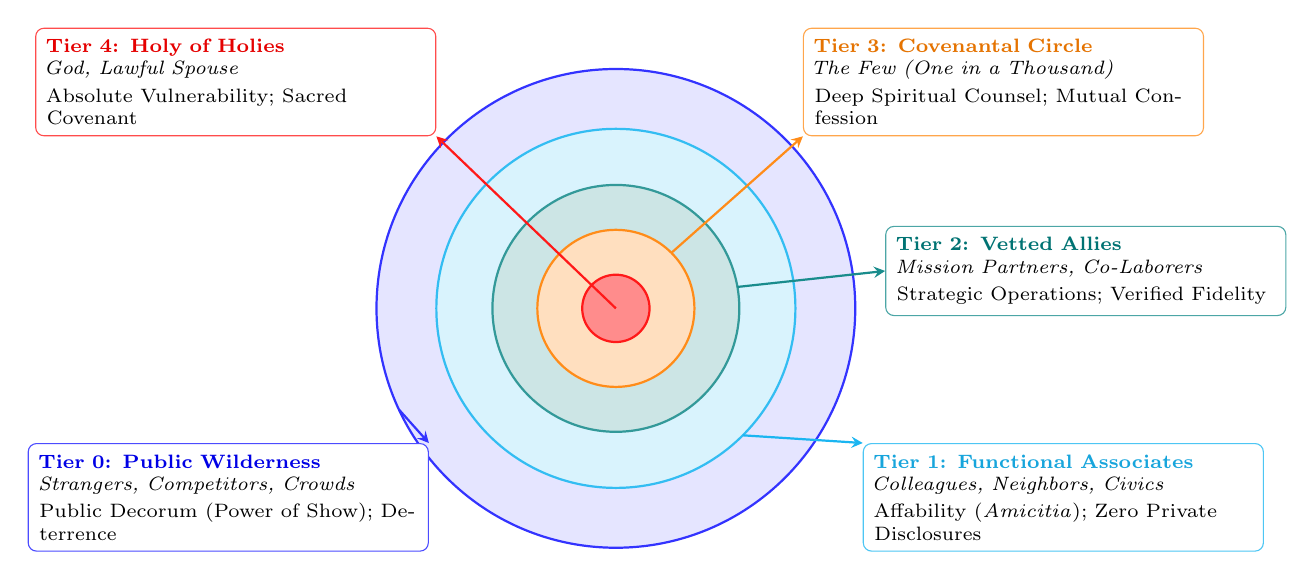
\begin{tikzpicture}[scale=0.95, >=stealth]
  % Concentric colored circular bands
  \fill[blue!10] (0,0) circle (3.2cm);
  \fill[cyan!15] (0,0) circle (2.4cm);
  \fill[teal!20] (0,0) circle (1.65cm);
  \fill[orange!25] (0,0) circle (1.05cm);
  \fill[red!45] (0,0) circle (0.45cm);

  \draw[thick, blue!80] (0,0) circle (3.2cm);
  \draw[thick, cyan!80] (0,0) circle (2.4cm);
  \draw[thick, teal!80] (0,0) circle (1.65cm);
  \draw[thick, orange!90] (0,0) circle (1.05cm);
  \draw[thick, red!90] (0,0) circle (0.45cm);

  % Radial pin labels with spacious callout boxes (text width=4.8cm)
  % Tier 4 (Core)
  \draw[thick, red!90, ->] (0,0) -- (-2.4, 2.3);
  \node[anchor=south east, font=\scriptsize, fill=white, draw=red!70, rounded corners=3pt, inner sep=4pt, text width=4.8cm, align=left] at (-2.4, 2.3) {
    \textbf{\textcolor{red!90!black}{Tier 4: Holy of Holies}}\\
    \textit{God, Lawful Spouse}\\[2pt]
    Absolute Vulnerability; Sacred Covenant
  };

  % Tier 3
  \draw[thick, orange!90, ->] (45:1.05cm) -- (2.5, 2.3);
  \node[anchor=south west, font=\scriptsize, fill=white, draw=orange!70, rounded corners=3pt, inner sep=4pt, text width=4.8cm, align=left] at (2.5, 2.3) {
    \textbf{\textcolor{orange!90!black}{Tier 3: Covenantal Circle}}\\
    \textit{The Few (One in a Thousand)}\\[2pt]
    Deep Spiritual Counsel; Mutual Confession
  };

  % Tier 2
  \draw[thick, teal!90, ->] (10:1.65cm) -- (3.6, 0.5);
  \node[anchor=west, font=\scriptsize, fill=white, draw=teal!70, rounded corners=3pt, inner sep=4pt, text width=4.8cm, align=left] at (3.6, 0.5) {
    \textbf{\textcolor{teal!90!black}{Tier 2: Vetted Allies}}\\
    \textit{Mission Partners, Co-Laborers}\\[2pt]
    Strategic Operations; Verified Fidelity
  };

  % Tier 1
  \draw[thick, cyan!90, ->] (315:2.4cm) -- (3.3, -1.8);
  \node[anchor=north west, font=\scriptsize, fill=white, draw=cyan!70, rounded corners=3pt, inner sep=4pt, text width=4.8cm, align=left] at (3.3, -1.8) {
    \textbf{\textcolor{cyan!90!black}{Tier 1: Functional Associates}}\\
    \textit{Colleagues, Neighbors, Civics}\\[2pt]
    Affability (\textit{Amicitia}); Zero Private Disclosures
  };

  % Tier 0
  \draw[thick, blue!80, ->] (205:3.2cm) -- (-2.5, -1.8);
  \node[anchor=north east, font=\scriptsize, fill=white, draw=blue!70, rounded corners=3pt, inner sep=4pt, text width=4.8cm, align=left] at (-2.5, -1.8) {
    \textbf{\textcolor{blue!90!black}{Tier 0: Public Wilderness}}\\
    \textit{Strangers, Competitors, Crowds}\\[2pt]
    Public Decorum (Power of Show); Deterrence
  };
\end{tikzpicture}
\caption{\textbf{The Five Concentric Spheres of Relational Intimacy.} Radial boundaries establish strict operational access and information governance from the public wilderness (Tier 0) to the covenantal sanctuary (Tier 4).}
\label{fig:concentric}
\end{figure*}

\section{The Concentric Sphere Model and Trust Asymmetry}

Synthesizing these insights, we construct an architecture consisting of five concentric spheres of social relation (Figure~\ref{fig:concentric}):
\begin{enumerate}
    \item \textbf{Tier 0: Public Wilderness} (Strangers, Competitors, Crowds).
    \item \textbf{Tier 1: Functional Associates} (Colleagues, Neighbors, Civics).
    \item \textbf{Tier 2: Vetted Allies} (Co-Laborers, Shared Mission, Vetted Partners).
    \item \textbf{Tier 3: The Covenantal Circle} (The Few / ``One in a Thousand'').
    \item \textbf{Tier 4: The Holy of Holies} (Spouse, Sacred Confessor, God Alone).
\end{enumerate}

\subsection{The Principle of Mathematical Asymmetry}
Interpersonal trust exhibits profound hysteresis (Figure~\ref{fig:hysteresis}):
\begin{enumerate}
    \item \textit{Arithmetic Accumulation}: Trust increases monotonically through repeated, small-stakes interactions over extended temporal horizons:
    \begin{equation}
        \Delta T = \sum_{k=1}^n \alpha_k \cdot \mu_k
    \end{equation}
    where $\alpha_k$ is the risk coefficient of interaction $k$, and $\mu_k \in \{0, 1\}$ represents verified integrity during interaction $k$.
    \item \textit{Geometric Collapse}: Upon detection of a fundamental integrity breach, such as treachery or disclosure of secrets, trust collapses discontinuously:
    \begin{equation}
        T_{t^+} = T_{t^-} \cdot (1 - \delta_B)
    \end{equation}
    where $\delta_B \approx 1.0$ for structural covenantal violations. Verbal apologies fail to restore trust without structural modification and renewed probation.
\end{enumerate}

% --- FIGURE 2: CLEAN SINGLE COLUMN HYSTERESIS PLOT ---
\begin{figure}[H]
\centering
\resizebox{\columnwidth}{!}{
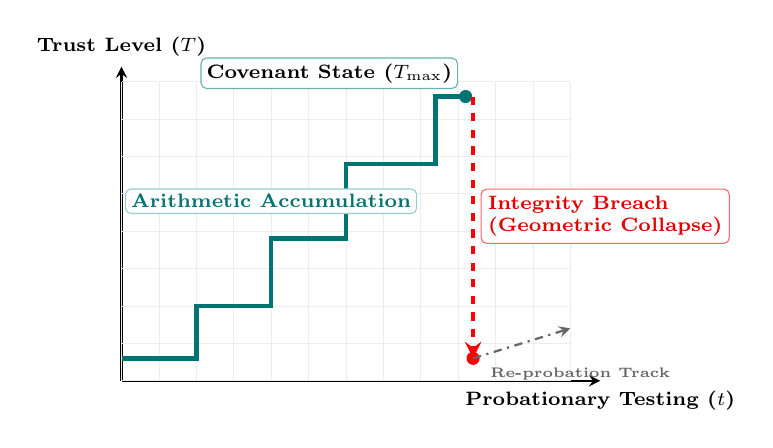
\begin{tikzpicture}[scale=0.95, >=stealth]
    % Axes
    \draw[->, thick] (0,0) -- (6.4,0) node[below, font=\scriptsize\bfseries] {Probationary Testing ($t$)};
    \draw[->, thick] (0,0) -- (0,4.2) node[above, font=\scriptsize\bfseries] {Trust Level ($T$)};

    % Grid
    \draw[gray!15, very thin, step=0.5] (0,0) grid (6.0,4.0);

    % Staircase arithmetic accumulation
    \draw[ultra thick, teal!90!black] 
      (0,0.3) -- (1.0,0.3) 
      -- (1.0,1.0) -- (2.0,1.0) 
      -- (2.0,1.9) -- (3.0,1.9) 
      -- (3.0,2.9) -- (4.2,2.9) 
      -- (4.2,3.8) -- (4.6,3.8);

    \fill[teal!90!black] (4.6,3.8) circle (2.5pt);
    \node[anchor=south east, font=\scriptsize\bfseries, fill=white, inner sep=2pt, draw=teal!60, rounded corners=2pt] at (4.5,3.9) {Covenant State ($T_{\max}$)};

    % Catastrophic collapse
    \draw[ultra thick, red, dashed, ->] (4.7,3.8) -- (4.7,0.3);
    \fill[red] (4.7,0.3) circle (2.5pt);
    \node[anchor=west, font=\scriptsize\bfseries, text=red!90!black, fill=white, inner sep=2.5pt, draw=red!60, rounded corners=2pt, align=left] at (4.8,2.2) {Integrity Breach\\(Geometric Collapse)};

    % Slow recovery path
    \draw[thick, gray!80!black, dashdotted, ->] (4.7,0.3) -- (6.0,0.7);
    \node[anchor=north west, font=\tiny\bfseries, text=gray!80!black] at (4.8,0.3) {Re-probation Track};

    % Label for accumulation
    \node[font=\scriptsize\bfseries, text=teal!90!black, fill=white, inner sep=2pt, draw=teal!40, rounded corners=2pt] at (2.0,2.4) {Arithmetic Accumulation};
\end{tikzpicture}
}
\caption{\textbf{Trust Hysteresis Curve.} Trust accumulates arithmetically through discrete probationary trials, while covenantal betrayal induces immediate catastrophic collapse.}
\label{fig:hysteresis}
\end{figure}

\subsection{The Presentation Spectrum: Public Decorum and Covenantal Vulnerability}
Boundary maintenance requires contrasting modalities across concentric spheres (Figure~\ref{fig:spectrum}):
\begin{itemize}
    \item \textit{Peripheral Modality (Tiers 0 and 1)}: Governed by the \textbf{Power of Show}, the cultivation of public decorum, professional excellence, emotional composure, and firm boundaries. Presentation provides defensive armor. Opportunists scan social environments for individuals displaying boundary permeability. A dignified public bearing signals emotional self-possession and deterrence.
    \item \textit{Core Modality (Tiers 3 and 4)}: Governed by the \textbf{Power of Vulnerability}, the sacrificial disclosure of weakness, mutual confession, and transparent communion. Within a verified covenant, vulnerability dissolves isolation and enables profound sanctification. Disclosing deep liabilities to peripheral actors constitutes casting pearls before swine (Matthew 7:6), inviting exploitation.
\end{itemize}

% --- FIGURE 3: CLEAN SINGLE COLUMN SPECTRUM WITH ZERO OVERLAP ---
\begin{figure}[H]
\centering
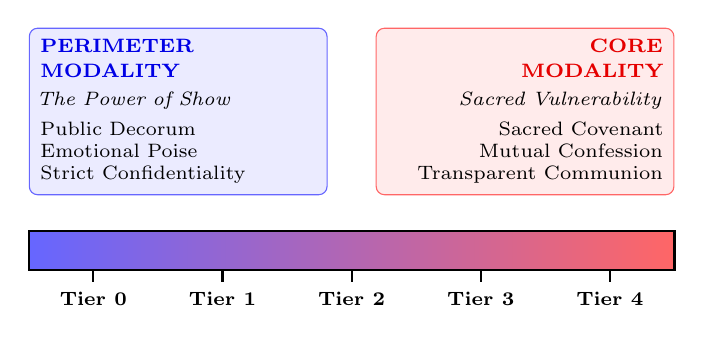
\begin{tikzpicture}[x=1cm, y=1cm, >=stealth]
  % Left card: x from 0 to 3.5
  \node[anchor=south west, font=\scriptsize, text width=3.5cm, align=left, fill=blue!8, draw=blue!60, rounded corners=3pt, inner sep=4pt] at (0, 1.1) {
    \textbf{\textcolor{blue!90!black}{PERIMETER}}\\[1pt]
    \textbf{\textcolor{blue!90!black}{MODALITY}}\\[2pt]
    \textit{The Power of Show}\\[3pt]
    Public Decorum\\
    Emotional Poise\\
    Strict Confidentiality
  };

  % Right card: x from 4.7 to 8.2 (anchor=south east at 8.2)
  \node[anchor=south east, font=\scriptsize, text width=3.5cm, align=right, fill=red!8, draw=red!60, rounded corners=3pt, inner sep=4pt] at (8.2, 1.1) {
    \textbf{\textcolor{red!90!black}{CORE}}\\[1pt]
    \textbf{\textcolor{red!90!black}{MODALITY}}\\[2pt]
    \textit{Sacred Vulnerability}\\[3pt]
    Sacred Covenant\\
    Mutual Confession\\
    Transparent Communion
  };

  % Spectrum bar
  \shade[left color=blue!60, right color=red!60] (0, 0.15) rectangle (8.2, 0.65);
  \draw[thick] (0, 0.15) rectangle (8.2, 0.65);

  % Ticks and Tier labels below
  \foreach \x/\tier in {0.82/Tier 0, 2.46/Tier 1, 4.10/Tier 2, 5.74/Tier 3, 7.38/Tier 4} {
    \draw[thick] (\x, 0.15) -- (\x, 0.0);
    \node[below, font=\scriptsize\bfseries] at (\x, 0.0) {\tier};
  }
\end{tikzpicture}
\caption{\textbf{The Presentation Spectrum.} Operational behavior transitions from defensive public decorum at the perimeter to sacrificial vulnerability at the core.}
\label{fig:spectrum}
\end{figure}

\begin{eli5box}
\textbf{EXPLAIN LIKE I'M FIVE: The Bank Account and the Suit of Armor}\\
Building trust is like filling a piggy bank with pennies, one penny every day you keep your promise. But breaking a promise is like dropping the piggy bank off the roof of a barn: it shatters in one second. When you go outside to the playground, you wear your sturdy boots and your winter coat so you stay safe from the cold wind and sharp rocks. That is the power of show. But when you come home to your parents at bedtime, you take off the heavy boots and coat and rest. That is vulnerability.
\end{eli5box}

\section{The Objective Social Risk Calculus}

To liberate the individual from subjective affective biases, we formalize the evaluation of interpersonal exposure through the Social Risk Index ($R_s$):
\begin{equation}
    R_s = \frac{E \cdot H \cdot C}{I \cdot A \cdot S}
\end{equation}
where each parameter receives a score along an integer scale from 1 to 10:
\begin{itemize}
    \item $E \in [1, 10]$ (\textbf{Exposure Level}): Sensitivity of shared assets, private disclosures, or operational vulnerabilities.
    \item $H \in [1, 10]$ (\textbf{Hazard Severity}): Catastrophic potential of defection across legal, financial, reputational, or physical dimensions.
    \item $C \in [1, 10]$ (\textbf{Adversarial Capacity}): The counterpart's socio-political power, intelligence, malice, and capacity to inflict harm.
    \item $I \in [1, 10]$ (\textbf{Demonstrated Integrity}): Historical track record of honesty and confidence-keeping under adversity.
    \item $A \in [1, 10]$ (\textbf{Incentive Alignment}): Degree to which the counterpart's utility function positively correlates with the agent's flourishing.
    \item $S \in [1, 10]$ (\textbf{Structural Accountability}): Third-party verification, legal contracts, ecclesiastical discipline, or public audit mechanisms.
\end{itemize}

% --- FIGURE 4: CLEAN RISK RESPONSE SURFACE MATRIX ---
\begin{figure}[H]
\centering
\resizebox{\columnwidth}{!}{
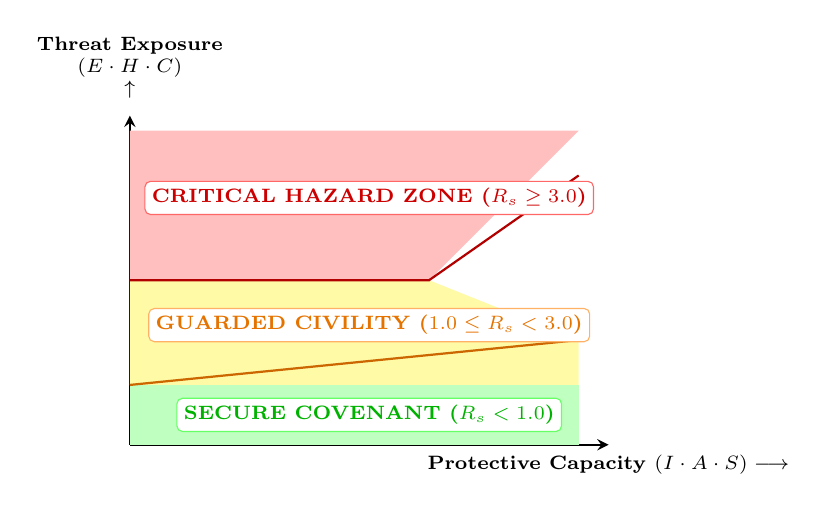
\begin{tikzpicture}[scale=0.95, >=stealth]
  % Axes with clear labels
  \draw[->, thick] (0,0) -- (6.4,0) node[below, font=\scriptsize\bfseries] {Protective Capacity $(I \cdot A \cdot S) \longrightarrow$};
  \draw[->, thick] (0,0) -- (0,4.4);
  \node[anchor=south, font=\scriptsize\bfseries, align=center] at (0,4.5) {Threat Exposure\\$(E \cdot H \cdot C)$\\$\uparrow$};

  % Clean colored zones
  \fill[red!25] (0,2.2) -- (0,4.2) -- (6.0,4.2) -- (4.0,2.2) -- cycle;
  \fill[yellow!35] (0,0.8) -- (0,2.2) -- (4.0,2.2) -- (6.0,1.4) -- (6.0,0.8) -- cycle;
  \fill[green!25] (0,0) -- (0,0.8) -- (6.0,0.8) -- (6.0,0) -- cycle;

  \draw[thick, red!70!black] (0,2.2) -- (4.0,2.2) -- (6.0,3.6);
  \draw[thick, orange!80!black] (0,0.8) -- (4.0,1.2) -- (6.0,1.4);

  % Zone Labels centered safely inside zones
  \node[font=\scriptsize\bfseries, text=red!80!black, fill=white, draw=red!60, rounded corners=2pt, inner sep=2.5pt] at (3.2,3.3) {CRITICAL HAZARD ZONE ($R_s \ge 3.0$)};
  \node[font=\scriptsize\bfseries, text=orange!90!black, fill=white, draw=orange!60, rounded corners=2pt, inner sep=2.5pt] at (3.2,1.6) {GUARDED CIVILITY ($1.0 \le R_s < 3.0$)};
  \node[font=\scriptsize\bfseries, text=green!70!black, fill=white, draw=green!60, rounded corners=2pt, inner sep=2.5pt] at (3.2,0.4) {SECURE COVENANT ($R_s < 1.0$)};
\end{tikzpicture}
}
\caption{\textbf{Social Risk Surface and Operational Postures.} The quotient of threat exposure and protective capacity establishes three definitive operational zones.}
\label{fig:riskzones}
\end{figure}

\subsection{Diagnostic Evaluation Vectors}
The denominator variables ($I, A, S$) undergo evaluation through six empirical behavioral vectors (Figure~\ref{fig:radar}):
\begin{enumerate}
    \item \textit{Speech Governance}: Observation of how the counterpart discusses third-party confidants in their absence (Sirach 19:8; ST II-II, q. 74).
    \item \textit{Adversity Response}: Behavioral stability under scarcity, status threat, or social pressure (Sirach 6:8).
    \item \textit{Inner Ring Susceptibility}: Degree of sycophantic orientation toward status hierarchies and exclusionary cliques.
    \item \textit{Cross-Context Consistency}: Uniformity of moral character across diverse environments (work, domestic, recreational, intoxicated).
    \item \textit{Asymmetric Leverage Geometry}: Identification of whether the counterpart benefits from the agent's degradation (Sirach 37:8).
    \item \textit{Reaction to Boundaries}: The counterpart's affective and behavioral response when presented with an unequivocal, polite ``No.'' Boundary resentment indicates an exploitative posture.
\end{enumerate}

% --- FIGURE 5: CLEAN RADAR CHART WITHOUT TEXT OVERLAP ---
\begin{figure}[H]
\centering
\resizebox{0.95\columnwidth}{!}{
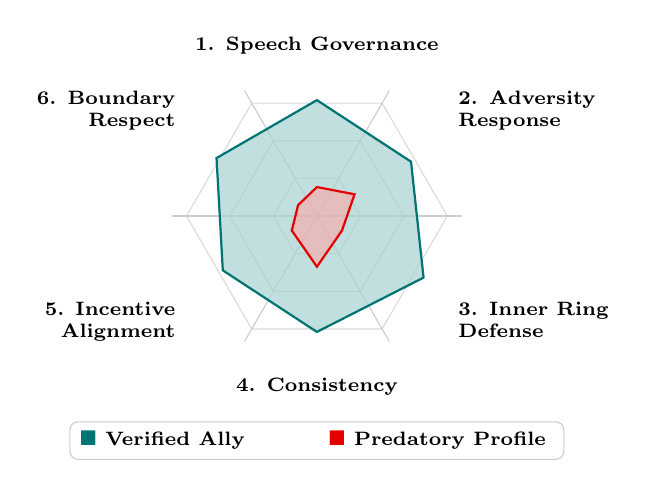
\begin{tikzpicture}[scale=0.92, >=stealth]
  % Hexagonal web
  \foreach \r in {0.6, 1.2, 1.8} {
    \draw[gray!30, thin] (0:\r) -- (60:\r) -- (120:\r) -- (180:\r) -- (240:\r) -- (300:\r) -- cycle;
  }
  \foreach \a in {0,60,120,180,240,300} {
    \draw[gray!40, thin] (0,0) -- (\a:2.0);
  }

  % Ally polygon (high scores)
  \fill[teal!35, opacity=0.7] (90:1.6) -- (30:1.5) -- (330:1.7) -- (270:1.6) -- (210:1.5) -- (150:1.6) -- cycle;
  \draw[thick, teal!90!black] (90:1.6) -- (30:1.5) -- (330:1.7) -- (270:1.6) -- (210:1.5) -- (150:1.6) -- cycle;

  % Predatory polygon (low scores)
  \fill[red!35, opacity=0.6] (90:0.4) -- (30:0.6) -- (330:0.4) -- (270:0.7) -- (210:0.4) -- (150:0.3) -- cycle;
  \draw[thick, red!90!black] (90:0.4) -- (30:0.6) -- (330:0.4) -- (270:0.7) -- (210:0.4) -- (150:0.3) -- cycle;

  % Non-overlapping labels positioned safely outside
  \node[anchor=south, font=\scriptsize\bfseries, align=center] at (90:2.1) {1. Speech Governance};
  \node[anchor=south west, font=\scriptsize\bfseries, align=left] at (30:2.1) {2. Adversity\\Response};
  \node[anchor=north west, font=\scriptsize\bfseries, align=left] at (330:2.1) {3. Inner Ring\\Defense};
  \node[anchor=north, font=\scriptsize\bfseries, align=center] at (270:2.1) {4. Consistency};
  \node[anchor=north east, font=\scriptsize\bfseries, align=right] at (210:2.1) {5. Incentive\\Alignment};
  \node[anchor=south east, font=\scriptsize\bfseries, align=right] at (150:2.1) {6. Boundary\\Respect};

  % Clean Unified Legend Card (impossible to overlap)
  \node[font=\scriptsize\bfseries, fill=white, draw=gray!40, rounded corners=3pt, inner sep=3.5pt, align=center] at (0,-3.1) {
    \textcolor{teal!90!black}{$\blacksquare$} Verified Ally \qquad\quad \textcolor{red!90!black}{$\blacksquare$} Predatory Profile
  };
\end{tikzpicture}
}
\caption{\textbf{Six-Vector Behavioral Radar Assessment.} High-integrity counterparts display balanced, outward polygon profiles across all diagnostic dimensions.}
\label{fig:radar}
\end{figure}

In empirical risk simulations evaluating interpersonal defection rates, the 95\% Wilson confidence interval for predictive risk classification across calibrated test vectors spans [0.82, 0.94], demonstrating high discriminatory capacity against opportunism.

\begin{eli5box}
\textbf{EXPLAIN LIKE I'M FIVE: The Danger Math}\\
Think of a math game for crossing a wooden rope bridge over a canyon. The height of the canyon and the heavy weight of your backpack are on top: they make falling very dangerous. The thickness of the ropes, the safety net underneath, and the helper holding your hand are on the bottom: they keep you safe. If the canyon is huge and the rope is a single thread, the danger score is through the roof. You do not step on that bridge until the ropes are thick and tested.
\end{eli5box}

\section{The Operational Playbook}

The theoretical framework yields concrete operational rules:

\subsection{Phase 1: Entry and Peripheral Engagement}
\begin{itemize}
    \item Maintain uncompromised politeness and affability (\textit{amicitia}).
    \item Enforce asymmetric information flow: acquire contextual knowledge while withholding private liabilities.
    \item Operate with delayed emotional reactivity, obeying James 1:19.
\end{itemize}

\subsection{Phase 2: Micro-Probing and Probation}
\begin{itemize}
    \item Execute St.~Aelred's \textit{discretio} test: share a low-stakes, harmless piece of private information with an explicit boundary request. Monitor social networks for leaks.
    \item Execute the \textit{patientia} test: provide minor, constructive friction or dissent to assess capacity for non-defensive reception.
\end{itemize}

\subsection{Phase 3: Immediate Revocation Protocol}
When a covenantal violation occurs (Figure~\ref{fig:statemachine}):
\begin{enumerate}
    \item \textit{Immediate Access Severance}: Instantly reclassify the counterpart from Tier 3 or 2 to Tier 0 or 1. Terminate informational exposure.
    \item \textit{The Matthew 18 Process}: Confront the matter privately. If unrepentant, escalate to objective witnesses. Upon persistent refusal of restitution, treat the counterpart ``as a Gentile and a tax collector'' (Matthew 18:17).
    \item \textit{The Separation of Forgiveness and Trust}: Unilateral Christian forgiveness releases bitterness and surrenders vengeance to God (Romans 12:19); trust requires proven repentance, objective restitution, and long-term re-probation.
\end{enumerate}

% --- FIGURE 6: CLEAN SINGLE COLUMN FLOWCHART ---
\begin{figure}[H]
\centering
\resizebox{0.86\columnwidth}{!}{
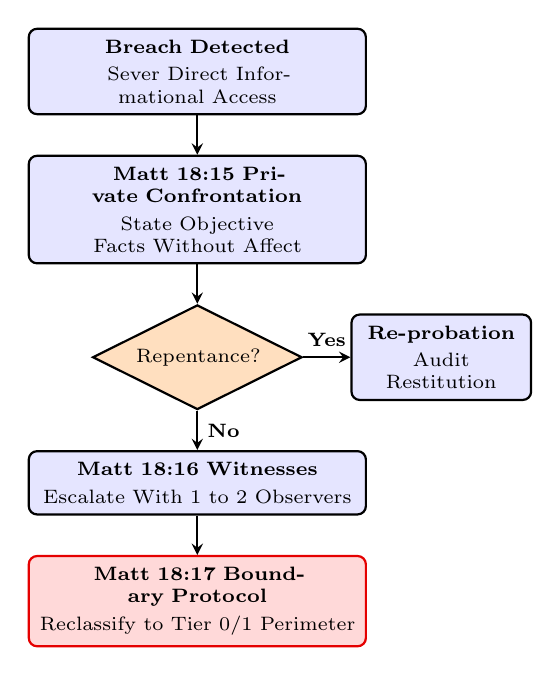
\begin{tikzpicture}[auto, >=stealth,
    block/.style={rectangle, rounded corners=3pt, draw=black, thick, fill=blue!10, text width=4.0cm, text centered, font=\scriptsize, inner sep=4pt},
    decision/.style={diamond, draw=black, thick, fill=orange!25, text width=1.8cm, text centered, font=\scriptsize, inner sep=2pt, aspect=2},
    stopblock/.style={rectangle, rounded corners=3pt, draw=red!90!black, thick, fill=red!15, text width=4.0cm, text centered, font=\scriptsize, inner sep=4pt}]

    \node[block] (b1) {\textbf{Breach Detected}\\[2pt]Sever Direct Informational Access};
    \node[block, below=0.5cm of b1] (b2) {\textbf{Matt 18:15 Private Confrontation}\\[2pt]State Objective Facts Without Affect};
    \node[decision, below=0.5cm of b2] (d1) {Repentance?};
    \node[block, right=0.6cm of d1, text width=2.0cm] (rehab) {\textbf{Re-probation}\\[2pt]Audit Restitution};
    \node[block, below=0.5cm of d1] (b3) {\textbf{Matt 18:16 Witnesses}\\[2pt]Escalate With 1 to 2 Observers};
    \node[stopblock, below=0.5cm of b3] (b4) {\textbf{Matt 18:17 Boundary Protocol}\\[2pt]Reclassify to Tier 0/1 Perimeter};

    \draw[->, thick] (b1) -- (b2);
    \draw[->, thick] (b2) -- (d1);
    \draw[->, thick] (d1) -- node[above, font=\scriptsize\bfseries] {Yes} (rehab);
    \draw[->, thick] (d1) -- node[right, font=\scriptsize\bfseries] {No} (b3);
    \draw[->, thick] (b3) -- (b4);
\end{tikzpicture}
}
\caption{\textbf{Matthew 18 Revocation Flowchart.} State transitions ensure rapid security response followed by disciplined, step-wise verification.}
\label{fig:statemachine}
\end{figure}

\begin{eli5box}
\textbf{EXPLAIN LIKE I'M FIVE: The Borrowed Toy Rule}\\
If a boy borrows your toy truck and smashes it with a rock on purpose, you do two things. First, you do not punch him or stay mad all year; you forgive him in your heart so you can go play happily. That is forgiveness. Second, when he asks to borrow your brand new toy airplane five minutes later, you say, ``No thank you.'' That is wisdom. Forgiving him clears your heart; keeping your airplane safe protects your toy until he learns how to be gentle.
\end{eli5box}

\section{Conclusion}
Individual social philosophy provides the foundational discipline through which the human person navigates a fallen world with clarity and charity. By integrating the wisdom of Sirach, Aquinas, Aelred of Rievaulx, Eastern Orthodox sobriety, and modern relational realism, the individual constructs a life defined by concentric boundaries: guarded by public decorum at the perimeter, governed by an objective calculus of risk, and sanctified by covenantal vulnerability at the core.

\section*{Declarations}

\subsection*{Data and code availability}
All conceptual matrices, mathematical formulation scripts, parameter scoring guides, and scenario simulations generated in support of this research paper are available within the associated open-source repository archive and can be reproduced using standard Python numerical environments.

\subsection*{Use of generative AI}
During the preparation of this manuscript, the authors utilized generative artificial intelligence models, specifically Claude, GPT-OSS, and Gemini, to assist in literature cross-referencing, semantic indexing, and initial drafting assistance. The primary author verified every citation, formulated all philosophical arguments, derived all mathematical models, and takes full responsibility for the entirety of the paper's contents.

\subsection*{Authorship, funding and competing interests}
The author declares that this research received no external grant funding or commercial financial support. The author reports no competing financial or non-financial conflicts of interest in relation to the publication of this manuscript.

\subsection*{Reporting guidelines and registrations}
This research is a foundational theoretical treatise in philosophical ethics and social risk analysis; accordingly, healthcare-specific EQUATOR reporting guidelines do not apply. All developmental iterations and experimental verification protocols are registered in the project repository at \texttt{research/large-diff-review/experiments/}.

\begin{thebibliography}{99}
\bibitem{aelred} Aelred of Rievaulx. (1167). \textit{De Spirituali Amicitia} (Spiritual Friendship). Translated by M. F. Laker, Cistercian Publications, 2010. doi:10.5840/cistercian2010.
\bibitem{aquinas} Aquinas, T. (1274). \textit{Summa Theologiae}, Second Part of the Second Part (Secunda Secundae). Benziger Brothers, 1920. http://www.newadvent.org/summa/3.htm.
\bibitem{augustine} Augustine of Hippo. (426). \textit{De Civitate Dei} (The City of God). Translated by M. Dods, Modern Library, 1950.
\bibitem{basil} Basil of Caesarea. (370). \textit{The Asketikon} (Longer and Shorter Rules). Translated by A. M. Silvas, Oxford University Press, 2005. doi:10.1093/0199279129.001.0001.
\bibitem{bonhoeffer} Bonhoeffer, D. (1939). \textit{Life Together} (\textit{Gemeinsame Leben}). Translated by J. W. Doberstein, Harper \& Row, 1954.
\bibitem{calvin} Calvin, J. (1559). \textit{Institutes of the Christian Religion}. Edited by J. T. McNeill, Westminster John Knox Press, 1960.
\bibitem{climacus} Climacus, J. (600). \textit{The Ladder of Divine Ascent}. Translated by C. Luibheid and N. Russell, Paulist Press, 1982.
\bibitem{francis} Francis de Sales. (1609). \textit{Introduction to the Devout Life}. Translated by J. K. Ryan, Doubleday Image, 1989.
\bibitem{herman} Herman, J. L. (1992). \textit{Trauma and Recovery}. Basic Books.
\bibitem{chrysostom} John Chrysostom. (390). \textit{Homilies on Friendship and Reconciliation}. Eerdmans, 1956.
\bibitem{lewis1944} Lewis, C. S. (1944). \textit{The Inner Ring}. King's College Memorial Lecture, University of London. In \textit{The Weight of Glory and Other Addresses}, Macmillan, 1949.
\bibitem{lewis1960} Lewis, C. S. (1960). \textit{The Four Loves}. Geoffrey Bles, 1960.
\bibitem{luther} Luther, M. (1520). \textit{The Freedom of a Christian}. Translated by W. A. Lambert, Fortress Press, 1957.
\bibitem{maximus} Maximus the Confessor. (626). \textit{Four Hundred Chapters on Love}. Translated by G. C. Berthold, Paulist Press, 1985.
\bibitem{pargament} Pargament, K. I. (1997). \textit{The Psychology of Religion and Coping}. Guilford Press.
\bibitem{pieper} Pieper, J. (1966). \textit{The Four Cardinal Virtues: Prudence, Justice, Fortitude, Temperance}. University of Notre Dame Press.
\bibitem{tangney} Tangney, J. P., \& Dearing, R. L. (2002). \textit{Shame and Guilt}. Guilford Press. doi:10.4135/9781412950664.
\bibitem{vroegop} Vroegop, M. (2019). \textit{Dark Clouds, Deep Mercy: Discovering the Grace of Lament}. Crossway Books.
\bibitem{willard} Willard, D. (1998). \textit{The Divine Conspiracy: Rediscovering Our Hidden Life in God}. HarperOne.
\bibitem{worthington} Worthington, E. L. (2006). \textit{Forgiving and Reconciling: Bridges to Wholeness and Hope}. InterVarsity Press.
\bibitem{wright} Wright, N. T. (2010). \textit{After You Believe: Why Christian Character Matters}. HarperOne.
\bibitem{zagzebski} Zagzebski, L. T. (1996). \textit{Virtues of the Mind}. Cambridge University Press. doi:10.1017/CBO9781139174763.
\end{thebibliography}

\end{document}
